\documentclass[11pt,a4paper,titlepage]{report}


% Document settings

\title{OSP Portfolio \\ Team $\langle$sql injection$\rangle$}

\author{
  Neil Ang\\
  \texttt{s3251533}
  \and
  ``Alfred" Yang Yuan\\
  \texttt{s3363619}
  \and
  Val Lyashov\\
  \texttt{s3366222}
}

\date{Semester 2, 2013}


% Change section numbering
%\renewcommand\thesection{\Roman{section}}
%\renewcommand\thesubsection{\Alph{subsection}}
\renewcommand\thesection{\arabic{section}}
\renewcommand\thesubsection{\thesection.\arabic{subsection}}


% Enable smart quotes
\usepackage [english]{babel}
\usepackage [autostyle]{csquotes}
\MakeOuterQuote{"}

% Alias pi name
\usepackage{xspace}
\newcommand{\rpi}{\textit{Raspberry Pi\textsuperscript{\textregistered}}}
\newcommand{\rpis}{\textit{Raspberry Pi\textsuperscript{\textregistered}s}}

% Side by side graphics
\usepackage{graphicx}
\usepackage{caption}
\usepackage{subcaption}

% Switch to biblatex
\usepackage{biblatex}
\bibliography{computer-vision}
\bibliography{audio}
\bibliography{servo}

% Add the bib to the toc
\DefineBibliographyStrings{english}{
  bibliography = {Bibliography},
}

% Better table height
\usepackage{tabu}

% The appendix
\usepackage{appendix}
\usepackage{pdfpages}


% Code highlighting
\usepackage{listings}

\lstset{
    language=C++,
    basicstyle=\small\sffamily,
    numbers=left,
    numberstyle=\tiny,
    frame=tb,
    columns=fullflexible,
    showstringspaces=false
}


% For links
\usepackage{hyperref}



% For marking what's left to do
\usepackage{color}


\begin{document}


\maketitle

\pagebreak
\tableofcontents
\thispagestyle{empty}
\pagebreak

\section{Introduction}

Live presentations audio recording is a well known problem for organisers, speakers and attendees alike. While there are significant amount of solutions available, factors such as cost, complexity and portability often limit widespread adoption. While existing services such as Echo360 and Lectopia work very well in recoding in a lecture theatre environment, ad-hoc deployment in smaller venues can be costly and logistically difficult to achieve.
 
In this project we present a cost-effective, light-weight presentation recording solution that requires little setup time. Designed with flexibility and rapid ad-hoc deployment as the guiding imperatives, the solution presents a good alternative for both personal and organisational use.


\section{Goals and Objectives}


The focus of the project has been to deliver an easy-to-use, fast to setup, and cost-effective solution to live presentation recording. The following table provides an overview of the core goals and projective we have strived towards over the course of the product development. The priority figure is the value on a scale of 1 to 5 (low to high respectively) that the design team have placed on the goal/objective (particularly during the initial prototype phase).


\textcolor{red}{TODO: Add table ref. Add learning objective goals.}

\begin{center}
\begin{table}
\begin{tabular}{|l|p{6cm}|c|}
    \hline
    \textbf{Goal / Objective} & \textbf{Description} & \textbf{Priority} \\ \hline
    Cost-effectiveness & One of the main factors that determines the viability of the end-product is the overall cost effectiveness. The aim is to provide a sub-\$200 product in a self-assembly state. & 5  \\ \hline
    
    Ease of use & The product has to be easy to use and operate by end-users. This includes setup, operation, troubleshooting stages of use. Some technical knowledge would be a required for the current form of the product. & 4  \\ \hline
    
    Semi-portability & As the project aims to primarily cater for ad-hoc recording scenarios, portability plays an important part of the overall system design. This takes form in complexity of assembly, size and weight of the finished product, the power usage and requirement, as well as the storage capacity of the recording functionality.& 3  \\ \hline

    Off-the-shelf hardware & To make the final product accessible to the largest share of prospective audience, the availability of components that make up the product becomes critical for the commercialisation of the project.& 2   \\ \hline

    Modularity & Partially related to the off-the-shelf hardware objective, modularity of components and accessories would ensure greater usage and types of operating environments the product can be deployed in.& 3  \\ \hline



\end{tabular}
\end{table}
\end{center}

\section{Feedback and Self-Reflection}

\subsection{Self Assessment}


\textcolor{red}{TODO: As a group we are very proud...}

\subsection{Summary of Prototype Demonstration}

Due to the hard work of all team members we were able to demonstrate a working prototype in our Week 10 laboratory. The presented product included an auto-startup feature so no laptop or router were needed for setup. We were able to successfully demonstrate to the class our face tracking, audio recording and motion sensing components of the solution. 

Although what we presented was a cutdown version of what was proposed in the project specification (missing the speech-to-text translation), we were very proud of what we had achieved and the positive reception the project received from our peers.

In preparation for the  demonstration we developed a short slide show, written speech and summary handout. All of these are available in the appendix. We also created a video of the working product incase we encountered technical issues during live demo. 

See the video here: \url{http://www.youtube.com/watch?v=hckEBpT1VcU}



\subsection{Peer Review Summary}

\textcolor{red}{This is waiting on the lab instructor to give us back our peer-review sheets.}


\subsection{Self Reflection / Lessons Learned}

\textcolor{red}{Individual responses here...}


\subsection{Description of how each learning objective is addressed}


Over the course of the project development, this team have made significant leaps in their knowledge of computer-hardware interfacing, operating system level functionality and application optimisation in a resource constrained environment. This section highlights how various learning objectives of the OSP course have been met.
 
\subsubsection{Learning Objective 1}
Over the course of the project, all of the ongoing development code has been managed through Github to ensure team members were always using the latest stable code when working on their assigned tasks.

With the face detection (computer vision) generating major CPU load when running on the Raspberry Pi, the team has gone through a significant amount of iterations of the functionality in order to achieve real-time response to the enviroment.


For efficiency during the initial development stages, most hardware interface interaction (e.g. servo controller, PIR sensor etc.) were prototyped using the Python programming language, and later ported into C when performance optimisation was required.


Debugging and performance has been used extensively over the course of the project for both hardware and software components. For Python, Pudb was the debugger of choice. For C/C++ Instruments and LLDB/GDB were utilised. On the hardware side, servo controller built-in error-checking was utilised for all communication to ensure hardware errors were caught and dealt with.
 


\section{Assumptions and Dependencies}
\section{General Constraints}
\section{Development Methodology}

\textcolor{red}{Reinforce how we met learning objective 1 here.}


\subsection{Programming languages}

\textcolor{red}{Python for prototyping, C/C++ for performance.}


\subsection{Development tools}

\subsection{Collaboration tools}

There were three main collaboration tools we used to progress this project: GitHub, Email and face-to-face meetings.

\subsubsection{GitHub}

From the start we setup a private\footnote{Access to this repository is available upon request.} git repository hosted on GitHub to store all our experimentation, development and production code. Since our project specification and portfolio were typeset in \LaTeX, we were also able to version control that as well. For all other project documentation (such as development logs and bibliography) we took advantage of GitHub's built in wiki to store this information.

GitHub worked for us because git was a version control system we all wanted to use, it was a tool we were familiar with, and it made it easy to identify when a piece of work had been completed.

\subsubsection{Email}

As postgraduate students, we all had competing priorities with our time which meant that we could not work together in person regularly. It was also difficult to meet due to the amount of hardware involved. As a result we often worked in isolation with very defined tasks.

So for us email was key for effective communication and delegating tasks. Once a week a group message was used to talk about our progress and goals for the coming week.

\subsubsection{Face-to-face meetings}

Being all together at once was a rare occasion and we had only a total of five out-of-class-hours group meetings that we all attended. We used the time to visually demonstrate what we had achieved with our tasks and discuss arising issues. 

If another group member was assigned to take over a task (e.g. handing over code to be optimised or integrated), we used this time to instruct in detail how the prototype code worked or how the hardware had been configured. 

\section{Difficulties Encountered}
\section{Architecture}
\subsection{System Design including configuration}
\subsection{Data Design}
\subsection{Program Design}


The software architecture for this project is basically a C/S (Client and Service) pattern. The server and client are connecting with Linux socket, using UDP protocol. The project has been divided into separated components, and after we build demo program for each part, we calculate the CPU usage, and than distribute the component into server and client.

In terms of components, they adopt messages to communicating with each other. That is to say, each component only cares about their own jobs, which improves the hoisin and independency for the system.

\textcolor{red}{TODO: Add communication digram here}


\subsubsection{Architecture Decisions}

\begin{center}
\begin{table}
\begin{tabular}{|p{0.3\textwidth}|p{0.2\textwidth}|p{0.5\textwidth}|}
    \hline
    \textbf{Aspects} & \textbf{Options} & \textbf{Decisions} \\ \hline
    
     Communication & 1. TCP \newline 2. UDP & 1. This is a small project that we only measure two PI communications, so the package loses shall happen in low possibility. \newline  2. In terms of complexity of communication, we do not need the message queue manages whether the message is delivered or not. \newline \textit{Option 2 adopted.
} \\ \hline

     Performance & 1. Idle \newline 2. Multiple threads & 1. There are brunches of components needs to wait communication messages to take next step. If we use idle function, it shall increase the queries between each component, dropping the system's cohesion. \newline  2. The worst case for face detection algorithm shall take a long time on detecting, dropping the system’s performance dramatically. \newline \textit{Option 2 adopted.
} \\ \hline

     Library & 1. Open CV \newline 2. PI face detection library & 1. Easy to debug on the laptop. \newline  2. Open CV library supports the USB camera, which can easily located on servo. \newline \textit{Option 1 adopted.
} \\ \hline
     
     Thread Communication & 1. Pipeline \newline 2. Sharing memory & 1. Sharing memory provides better performance on communication. \newline  2. There are too many components that need to communication, if we use pipeline, it shall increase the complex for the project and decrease the maintenance. \newline \textit{Option 2 adopted.
} \\ \hline
     
     Memory & 1. Instance every copy
 \newline 2. Copy on write & 1. All components may assess the message data. if every component create an instance, there shall be a lot memory waste for brunches of different instance for same object.
 \newline  2. Copy on write provides more performance; because it shall not spend too much time on copying the data form one object to another. \newline \textit{Option 2 adopted.
} \\ \hline

     Message scheduling & 1. FCFS \newline 2. More complex algorithms & 1. FCFS is easy to implement and maintain.
 \newline  2. This is an easy project, and every message may have same priority. \newline \textit{Option 1 adopted.
} \\ \hline

\end{tabular}
\end{table}
\end{center}


\textcolor{red}{TODO: Add sequence digram here}

\subsubsection{Sharing memory for threads communication}

All the threads have their own stack, but they shall share the heap memory. So we build all the service in heap memory. (use malloc) In addition,  in order for easy accessing from different threads, we allocate a pointer in static memory block that point to the heap. 

The code of Singleton is shown as below:

\textcolor{red}{TODO: INSERT CODE}


\subsubsection{Memory Scheduling}

The most different part for the message definition is that the length of the message does not know before it construct. However, we cannot create a big buffer because of the memory limited for the PI. As a result of that, I use a strategy only define 1 char array, and use malloc to increase the length dynamically.

The code of dynamical message length is shown as below:

\textcolor{red}{TODO: INSERT CODE}


\subsubsection{Copy on write}

PI has little memory size, so it is impossible to reallco memory for passing large frame data buffer that come from face detection frame. More specify, it turn to be waste of memory coping more than one instance of any kind of instance in the project. 

In order to reduce the usage of memory, we adopt the Copy on write strategy. This strategy only makes a copy when there is some modification on the object, and the most of time they shall only create a new pointer point to the original address.

The trade-off for this strategy is that it is no thread-safe, because more than one thread want to access the object when about to change the original data. However, in our project, all the processes, such as face detection and messages, are read-only process, which means that we do not have to consider race condition when we use this approach. 

The code of message is shown as below:


\textcolor{red}{TODO: INSERT CODE}

\subsubsection{Message serialization}

As the communication between server and client, we encode the message data into an array that uses '\textbackslash0' at the end. And the message array can also be encoded into message.

The code of message serialization is shown as below:

\textcolor{red}{TODO: INSERT CODE}


\subsubsection{Message queue class}

The message queue acts as the communication component in the system. All other components push message to the message queue and the dispatch messages to appropriate component. 

The most important functionality for message queue should be synchronization. That is to say, only one thread can push or pop message at the same time in order to prevent race condition. More specific, the message queue use conditional valuable to control the race condition. 

The core code of message queue is shown as below:

\textcolor{red}{TODO: INSERT CODE}


\subsubsection{FCFS strategy}

The code shows that we use the simplest strategy to scheduling the message, which means that when there is a message push into the message queue, the dispatching thread shall read the first message in the message queue send to the appropriate component to serve it. In addition, the dispatch thread shall be hinge up and wait when there are no messages in message queue.

The message shall be dispatched messages using design pattern: chain of responsibility. The process base on the message ID, which have been introduced in message protocol part. The dispatch component shall query message id and push the message to the serve components.

The core code of client message dispatching is shown as below:

\textcolor{red}{TODO: INSERT CODE}





\subsubsection{Software Design}

\subsubsection{Source code or patches for all original work.}


\subsubsection{Server Code}

\begin{lstlisting}[caption=basic-service.h,language=C++]
#ifndef __BASE_SERVICE_H__
#define __BASE_SERVICE_H__

#include "message.h"
#include "message_query.h"

class base_service {
public:

  virtual bool setUpService()  = 0;
  virtual void startMainLoop() = 0;
  virtual void stopMainLoop()  = 0;

  virtual void postMessage(Message *m)
  {
    MessageQuery::GetInstance()->pushMessage(m);
  }

  virtual void receiveMessage(const Message& m) = 0;
};

#endif
\end{lstlisting}





\begin{lstlisting}[caption=comm.h,language=C++]
#define LISTEN_THREAD 0
#define WRITE_THREAD  1
#define READ_THREAD   2
#define THREAD_NUM    3

#include <pthread.h>
#include "message_query.h"
#include "message.h"
#include <sys/socket.h>
#include <netinet/in.h>
#include <arpa/inet.h>
#include <stdio.h>
#include <stdlib.h>
#include <errno.h>
#include <string.h>
#include <time.h>
#include <unistd.h>

class Comm {
protected:

  struct sockaddr_in serv_addr;
  int server_socket;
  int client_socket;

  pthread_t threads[THREAD_NUM];
  int  thread_ids[THREAD_NUM];
  bool thread_running[THREAD_NUM];

public:

  MessageQuery *query;

public:

  Comm();
  ~Comm();

  void         createThreads();
  bool         isThreadRunning(int thread_index);

  int          sendMessage(Message *m);
  Message    * readMessage();
  virtual bool dispatchMessage(Message *m) = 0;
};

void         * writeThread(void *arg);
void         * readThread(void *arg);

\end{lstlisting}







\begin{lstlisting}[caption=comm.cpp,language=C++]
#include <sys/socket.h>
#include <netinet/in.h>
#include <arpa/inet.h>
#include <stdio.h>
#include <stdlib.h>
#include <errno.h>
#include <string.h>
#include <time.h>
#include <unistd.h>

#define BUFFER_SIZE 1024

#include <iostream>
using std::cout;        using std::endl;

#include "comm.h"

Comm::Comm()
{
  query = MessageQuery::GetInstance();
  memset(thread_running, 1, THREAD_NUM);
}

Comm::~Comm()
{}

void Comm::createThreads()
{
  thread_ids[WRITE_THREAD] = pthread_create(&threads[WRITE_THREAD],
                                            NULL,
                                            writeThread,
                                            this);

  thread_ids[READ_THREAD] = pthread_create(&threads[READ_THREAD],
                                           NULL,
                                           readThread,
                                           this);
}

bool Comm::isThreadRunning(int thread_index)
{
  return thread_running[thread_index];
}

int Comm::sendMessage(Message *m)
{
  void *p = m->messageData();

  write(client_socket, p, m->messageLength());
  free(p);
  return 0;
}

Message * Comm::readMessage()
{
  char buffer[BUFFER_SIZE] = { 0 };
  int  count               = 0;

  count         = read(client_socket, buffer, sizeof(buffer) - 1);
  buffer[count] = 0;
  Message *m = Message::createMessage(buffer);
  return m;
}

void* writeThread(void *arg)
{
  printf("write thread start\n");

  Comm *s = (Comm *)arg;
  char  buffer[BUFFER_SIZE];

  while (s->isThreadRunning(WRITE_THREAD))
  {
    memset(buffer, 0, BUFFER_SIZE);

    Message *m = MessageQuery::GetInstance()->popMessage();
    s->sendMessage(m);
    delete m;
  }
  return NULL;
}

void* readThread(void *arg)
{
  printf("read thread start\n");

  Comm *s = (Comm *)arg;

  while (s->isThreadRunning(READ_THREAD))
  {
    Message *m = s->readMessage();

    printf("%s\n", m->messageBodyData());

    if (s->dispatchMessage(m)) delete m;
  }
  return NULL;
}
\end{lstlisting}





\begin{lstlisting}[caption=face-detect.h,language=C++]
#include "singleton.h"
#include "base_service.h"
#include <string>
#include <opencv2/opencv.hpp>
using std::string;
using namespace cv;

struct face_detect_arg;
class Message;

class face_detect
  : public Singleton<face_detect>
    , public base_service {
  const char *strWindowName;
  const char *strCascadeClassifier;
  const int   nFrameWaitTime;

  bool isRunning;

  face_detect_arg *fd;

public:

  pthread_t face_main_thread;
  pthread_t face_detect_thread;
  const int nFrameWidth;
  const int nFrameHeight;

public:

  bool             isMainThreadRunning() const;
  const char     * getWindowName() const;
  face_detect_arg* getDetectArg();
  const int        getFrameWaitTime() const;
  const int        getFrameWidth() const;
  const int        getFrameHeight() const;

  pthread_t        getMainThread() const;
  pthread_t        getDetectThread() const;

public:

  face_detect();
  ~face_detect();

  virtual bool setUpService();
  virtual void startMainLoop();
  virtual void stopMainLoop();
  virtual void receiveMessage(const Message& m);

public:

  void       loadCascadeClassifier(const char        *strPath,
                                   CascadeClassifier *pc);
  CvCapture* createCaptureFrameCamera(int nCaptureIndex = -1);
  IplImage * captureFrame(CvCapture *pCapture);
};

struct face_detect_arg
{
  CascadeClassifier *pCvHaar;
  IplImage          *pImage;
  bool               bDetected;
  CvRect             rc;
  bool               threadRunning;
};

void * faceCaptureFunction(void *arg);
void * faceDetectFunction(void *arg);
CvRect detectFaceInImage(IplImage          *inputImg,
                         CascadeClassifier *cascade);

\end{lstlisting}








\begin{lstlisting}[caption=face-detect.cpp,language=C++]
#include <opencv2/opencv.hpp>
#include <string>
#include <iostream>
#include <vector>
#include <assert.h>
#include <pthread.h>
#include "face_detect.h"
#include "message.h"
#include "maestro.h"
#include <stdio.h>
using std::string;      using std::cout;
using std::endl;        using std::vector;
using std::cerr;
using namespace cv;

#define NA_FACE_MOVE_THRESHOLD 400
#define GUI_MODE 0

pthread_mutex_t mutex = PTHREAD_MUTEX_INITIALIZER;

#define FAILURE_CHECK(p, x)      \
  assert(p);                     \
  if (p == NULL)                 \
  {                              \
    std::cerr << x << std::endl; \
    exit(EXIT_FAILURE);          \
  }

face_detect::face_detect()
  : strWindowName("Face detection test")
    , strCascadeClassifier("lbpcascade_frontalface.xml")
    , nFrameWaitTime(33)
    , nFrameWidth(320)
    , nFrameHeight(240)
    , isRunning(false)
{}

face_detect::~face_detect()
{}

bool face_detect::setUpService()
{
  fd          = (face_detect_arg *)malloc(sizeof(face_detect_arg));
  fd->pCvHaar = new CascadeClassifier();
  loadCascadeClassifier(strCascadeClassifier, fd->pCvHaar);

  fd->pImage        = NULL;
  fd->threadRunning = true;
  fd->bDetected     = false;

  return true;
}

void face_detect::startMainLoop()
{
  isRunning = true;
  pthread_create(&face_main_thread, NULL, faceCaptureFunction, (void *)_instance);

  //	faceCaptureFunction((void*)this);
}

void face_detect::stopMainLoop()
{
  isRunning         = false;
  fd->threadRunning = false;
}

void face_detect::receiveMessage(const Message& m)
{
  // TODO: handle the message ...
}

void face_detect::loadCascadeClassifier(const char        *strPath,
                                        CascadeClassifier *pc)
{
  FAILURE_CHECK(pc, "Conldn't load classifier");

  if (!pc->load(strPath))
  {
    std::cerr << "Conldn't load classifier" << endl;
    exit(EXIT_FAILURE);
  }
}

CvCapture * face_detect::createCaptureFrameCamera(int nCaptureIndex)
{
  CvCapture *p = cvCaptureFromCAM(nCaptureIndex);

  FAILURE_CHECK(p, "Init Capture Failed");

  if (!cvGrabFrame(p))
  {
    std::cerr << "Conldn't GrabFrame" << std::endl;
    exit(EXIT_FAILURE);
  }

  cvSetCaptureProperty(p, CV_CAP_PROP_FRAME_WIDTH,  nFrameWidth);
  cvSetCaptureProperty(p, CV_CAP_PROP_FRAME_HEIGHT, nFrameHeight);
  cvSetCaptureProperty(p, CV_CAP_PROP_FPS,          5);

  return p;
}

IplImage * face_detect::captureFrame(CvCapture *pCapture)
{
  IplImage *p = cvQueryFrame(pCapture);

  FAILURE_CHECK(p, "Error: cvQueryFrame failed");

  return p;
}

CvRect detectFaceInImage(IplImage *inputImg, CascadeClassifier *cascade)
{

  CvSize minFeatureSize = cvSize(80, 80);

  int flags = CV_HAAR_FIND_BIGGEST_OBJECT | CV_HAAR_DO_ROUGH_SEARCH;

  float search_scale_factor = 1.1f;

  IplImage *detectImg = inputImg;

  if (detectImg->nChannels > 1)
  {
    CvSize size       = cvSize(detectImg->width, detectImg->height);
    IplImage *greyImg = cvCreateImage(size, IPL_DEPTH_8U, 1);
    cvCvtColor(detectImg, greyImg, CV_BGR2GRAY);
    detectImg = greyImg;
  }

  vector<Rect> rects;
  cascade->detectMultiScale(detectImg,
                            rects,
                            search_scale_factor,
                            3,
                            flags,
                            minFeatureSize);

  int nFaces = rects.size();

  CvRect rc = cvRect(-1, -1, -1, -1);

  if (nFaces > 0)
  {
    rc = cvRect(rects[0].x, rects[0].y, rects[0].width, rects[0].height);
  }

  if (detectImg->nChannels > 1) cvReleaseImage(&detectImg);

  return rc;
}

double euclideanDistance(CvPoint pt1, CvPoint pt2) {
  double x = pt1.x - pt2.x;
  double y = pt1.y - pt2.y;
  double dist;

  dist = pow(x, 2) + pow(y, 2);
  return dist;
}

void* faceCaptureFunction(void *arg)
{
  face_detect *fdc    = (face_detect *)arg;
  face_detect_arg *fd = fdc->getDetectArg();

  CvCapture *pCapture = fdc->createCaptureFrameCamera();

  IplImage *src =  cvQueryFrame(pCapture);

  pthread_create(&(fdc->face_detect_thread), NULL, faceDetectFunction,
                 (void *)fd);

  float screenDivisions = 2.6;

  Point rightPt2  = Point(fdc->nFrameWidth / screenDivisions,
                          fdc->nFrameHeight - 1);
  Point leftPt1   = Point(fdc->nFrameWidth - (fdc->nFrameWidth / screenDivisions),
                          0);
  Point topPt2    = Point(fdc->nFrameWidth - 1,
                          fdc->nFrameHeight / screenDivisions);
  Point bottomPt1 =
    Point(0, fdc->nFrameHeight - (fdc->nFrameHeight / screenDivisions));

  Maestro *maestro = Maestro::GetInstance();
  maestro->goHome(maestro->horizontalServo);
  maestro->goHome(maestro->verticalServo);
      usleep(1);

  CvPoint lastFace;
  lastFace.x = fdc->nFrameWidth / 2.0;
  lastFace.y = fdc->nFrameHeight / 2.0;

  CvRect rc;
  bool   bDetected = false;

  while (fdc->isMainThreadRunning())
  {
    IplImage *pImg = cvQueryFrame(pCapture);

    if (!pImg)
    {
      std::cerr << "Query Frame Failed" << endl;
      usleep(1000);
      continue;
    }

    assert(pImg);
    pthread_mutex_lock(&mutex);
    fd->pImage = pImg;
    bDetected  = fd->bDetected;
    rc         = fd->rc;
    pthread_mutex_unlock(&mutex);

    CvPoint facePoint;
    facePoint.x = 0;
    facePoint.y = 0;

    if (bDetected)
    {
      CvPoint p1 = cvPoint(rc.x, rc.y);
      CvPoint p2 = cvPoint(rc.x + rc.width, rc.y + rc.height);
      cvRectangle(pImg, p1, p2, CV_RGB(0, 255, 0), 5, 8);

      facePoint.x = rc.x + (rc.width / 2.0f);
      facePoint.y = rc.y + (rc.height / 2.0f);

        printf("Face Detected\n");
    }

    if ((facePoint.x > 0) && (facePoint.y > 0)) {
      double dist = euclideanDistance(facePoint, lastFace);

      if ((dist > 0) && (dist < NA_FACE_MOVE_THRESHOLD))
      {
        printf("send rotate command\n");

        if (facePoint.x < rightPt2.x) maestro->stepUp(maestro->horizontalServo);
        else if (facePoint.x > leftPt1.x) maestro->stepDown(
            maestro->horizontalServo);

        if (facePoint.y < topPt2.y) maestro->stepUp(maestro->verticalServo);

        else if (facePoint.y > bottomPt1.y) maestro->stepDown(
            maestro->verticalServo);
      }

      lastFace.x = facePoint.x;
      lastFace.y = facePoint.y;
    }

    if (cvWaitKey(fdc->getFrameWaitTime()) == 27) fdc->stopMainLoop();

    usleep(1);
  }

  cvReleaseCapture(&pCapture);
  return NULL;
}

void* faceDetectFunction(void *arg)
{
  face_detect_arg *fd = (face_detect_arg *)arg;

  while (fd->threadRunning)
  {
    if (fd->pImage == NULL)
    {
      continue;
    }

    pthread_mutex_lock(&mutex);
    IplImage *pImg = fd->pImage;
    pthread_mutex_unlock(&mutex);

    CvRect rc = detectFaceInImage(pImg, fd->pCvHaar);

    if (rc.x != -1)
    {
      pthread_mutex_lock(&mutex);
      fd->bDetected = true;
      fd->rc        = rc;
      pthread_mutex_unlock(&mutex);
    }
    else
    {
      pthread_mutex_lock(&mutex);
      fd->bDetected = false;
      pthread_mutex_unlock(&mutex);
    }
  }

  return NULL;
}

bool face_detect::isMainThreadRunning() const
{
  return isRunning;
}

const char * face_detect::getWindowName() const
{
  return strWindowName;
}

face_detect_arg * face_detect::getDetectArg()
{
  return fd;
}

pthread_t face_detect::getMainThread() const
{
  return face_main_thread;
}

pthread_t face_detect::getDetectThread() const
{
  return face_detect_thread;
}

const int face_detect::getFrameWaitTime() const
{
  return nFrameWaitTime;
}

const int face_detect::getFrameWidth() const
{
  return nFrameWidth;
}

const int face_detect::getFrameHeight() const
{
  return nFrameHeight;
}

\end{lstlisting}





\begin{lstlisting}[caption=maestro.h,language=C++]
#ifndef __maestro__
#define __maestro__

#include <iostream>
#include <string>
#include <stdio.h>
#include <unistd.h>
#include <fcntl.h>
#include <termios.h>

#include "singleton.h"
#include "base_service.h"

// Source:
// http://stackoverflow.com/questions/134569/c-exception-throwing-stdstring
struct MaestroException : public std::exception
{
  std::string s;
  MaestroException(std::string ss) : s(ss) {}

  ~MaestroException() throw() {}

  const char* what() const throw() {
    return s.c_str();
  }
};

#ifndef __servo__
# define __servo__

class Servo {
private:

  unsigned char  _channel;
  unsigned int   _min;
  unsigned int   _max;
  unsigned short _pos;
  unsigned short _home;

public:

  Servo(unsigned char c, unsigned int mn, unsigned int mx,
        unsigned int hm) : _channel(c), _min(mn), _max(mx), _home(hm) {}

  unsigned char getChannel() {
    return _channel;
  }

  unsigned short getHome() {
    return _home;
  }

  unsigned short getMin() {
    return _min;
  }

  unsigned short getMax() {
    return _max;
  }

  unsigned short getPos() {
    return _pos;
  }

  void setPos(unsigned short p) {
    _pos = p;
  }
};

#endif /* defined(__servo__) */

#ifdef __APPLE__
# define NA_DEVICE "/dev/cu.usbmodem00065291"
#else
# define NA_DEVICE "/dev/ttyACM0"
#endif // ifdef __APPLE__

class Maestro
  : public Singleton<Maestro>
    , public base_service {
private:

  const char *_device;
  int         _fd;

public:

  Servo *horizontalServo;
  Servo *verticalServo;

public:

  Maestro() : _device(NA_DEVICE) {}

  ~Maestro() {
    close(_fd);
  }

  int          getError(Servo *servo);
  int          goHome(Servo *);
  int          getPosition(Servo *);
  int          setPosition(Servo    *,
                           unsigned short);
  int          stepUp(Servo *);
  int          stepDown(Servo *);

  virtual bool setUpService();
  virtual void startMainLoop();
  virtual void stopMainLoop();
  virtual void receiveMessage(const Message& m);

private:

  void openDevice();
};

#endif // ifndef __maestro__

\end{lstlisting}





\begin{lstlisting}[caption=maestro.cpp,language=C++]
#include "maestro.h"
#define NA_STEP_VALUE 150

int Maestro::goHome(Servo *servo) {
  unsigned char command[] = { 0xA2, servo->getChannel() };

  if (write(_fd, command, sizeof(command)) == -1) {
    perror("error writing");
    return -1;
  }

  servo->setPos(servo->getHome());

  return 0;
}

int Maestro::getPosition(Servo *servo) {
  return (int)servo->getPos();
}

int Maestro::setPosition(Servo *servo, unsigned short target) {
  if (target > servo->getMax()) target = servo->getMax();

  if (target < servo->getMin()) target = servo->getMin();
  unsigned char command[] =
  { 0x84, servo->getChannel(), static_cast<unsigned char>(target & 0x7F),
    static_cast<unsigned char>(target >> 7 & 0x7F) };

  if (write(_fd, command, sizeof(command)) == -1) {
    perror("error writing");
    return -1;
  }

  servo->setPos(target);
  return 0;
}

int Maestro::stepUp(Servo *servo) {
  return setPosition(servo, getPosition(servo) + NA_STEP_VALUE);
}

int Maestro::stepDown(Servo *servo) {
  return setPosition(servo, getPosition(servo) - NA_STEP_VALUE);
}

#define KEYCONTROL 0

#if KEYCONTROL
# include <termios.h>
# include <unistd.h>
#endif // if KEYCONTROL

void Maestro::openDevice()
{
  _fd = open(_device, O_RDWR | O_NOCTTY);

  if (_fd == -1) {
    perror(_device);
    throw MaestroException("Invalid Device");
  }
}

bool Maestro::setUpService()
{
  openDevice();
  horizontalServo = new Servo(0, 3968, 9216, 6104);
  verticalServo   = new Servo(1, 3968, 9216, 8220);

  this->goHome(horizontalServo);
  this->goHome(verticalServo);
}

void Maestro::startMainLoop()
{}

void Maestro::stopMainLoop()
{}

void Maestro::receiveMessage(const Message& m)
{}

#undef NA_STEP_VALUE
\end{lstlisting}





\begin{lstlisting}[caption=main-server.cpp,language=C++]
#include "server.h"

int main(int argc, char **argv)
{
  Server *s = Server::GetInstance();

  s->setUpService();
  s->startMainLoop();

  return 0;
}
\end{lstlisting}





\begin{lstlisting}[caption=message.h,language=C++]
#ifndef __MESSAGE_H__
#define __MESSAGE_H__

#include <string>
using std::string;

#define TEST 0

enum message_id
{
  M_START = 0,
  M_END,
  M_DETECTED,
  M_UNDETECTED,

  M_PIR_DETECTED = 100,
  M_PIR_UN_DETECTED,

  M_BEGIN_AUDIO_RECORDING = 200,
  M_END_AUDIO_RECORDING,
};

enum message_handle_proxy
{
  proxy_server = 0,
  proxy_client,
};

struct message_head
{
  int mh_id;
  int mh_size;
  int mh_handle_proxy;
  int mh_reserve;
};

struct message_body
{
  int  mb_len;
  char mb_data[1];
};

struct message
{
  message_head *head;
  message_body *body;
};

class Server;

class Message {
  friend class Server;
#if TEST

public:

#endif // if TEST
  message *_impl;

public:

  Message();
  Message(const Message& other);
  Message& operator=(const Message& rhs);
  Message(void *data, int size);
  ~Message();

public:

  void            initMessage(int    id,
                              string message_data);
  int             messageLength() const;
  void          * messageData() const;
  char          * messageBodyData() const;
  int             getMessageHandleProxy(int id);

  static Message* createMessage(void *data);
};

#endif

\end{lstlisting}





\begin{lstlisting}[caption=message.cpp,language=C++]
#include "message.h"
#include <stdlib.h>
#include <stdio.h>
#include <string.h>

Message::Message()
{
  _impl       = new message();
  _impl->head = new message_head();
  _impl->body = (message_body *)malloc(sizeof(message_body));
}

Message::Message(const Message& other)
{
  _impl       = new message();
  _impl->head = new message_head();
  _impl->body = (message_body *)malloc(sizeof(message_body));

    memcpy(_impl, other._impl, sizeof(message));
}

Message& Message::operator=(const Message& rhs)
{
  if (&rhs != this)
  {
    _impl       = new message();
    _impl->head = new message_head();
    _impl->body = (message_body *)malloc(sizeof(message_body));

    memcpy(_impl, rhs._impl, sizeof(message));
  }

  return *this;
}

Message::~Message()
{
  delete _impl->head;
  delete _impl->body;
  delete _impl;
}

Message * Message::createMessage(void *data)
{
  Message *m = new Message();

  int *p = (int *)data;

  m->_impl->head->mh_id           = *(p + 0);
  m->_impl->head->mh_size         = *(p + 1);
  m->_impl->head->mh_handle_proxy = *(p + 2);
  m->_impl->head->mh_reserve      = *(p + 3);
  char *c   = (char *)((p + 4) + 1);
  int   len = strlen(c);
  m->_impl->body         = (message_body *)malloc(
    sizeof(char) * (len + 1) + sizeof(int));
  m->_impl->body->mb_len = *(p + 4);
    memcpy(m->_impl->body->mb_data, c, len);
  m->_impl->body->mb_data[len] = 0;

  return m;
}

void Message::initMessage(int id, string message_data)
{
  _impl->head->mh_id = id;

  _impl->head->mh_handle_proxy = getMessageHandleProxy(id);
  _impl->head->mh_reserve      = 0;

  _impl->body = (message_body *)malloc(sizeof(int) +
                                       sizeof(char) * (message_data.size() + 1));
  _impl->body->mb_len = message_data.size();
    memcpy(_impl->body->mb_data, message_data.c_str(), message_data.size());
  *(_impl->body->mb_data + message_data.size()) = 0;

  _impl->head->mh_size = sizeof(message_head) + sizeof(int)
                         + sizeof(char) * (message_data.size() + 1);
}

int Message::messageLength() const
{
  return _impl->head->mh_size;
}

void * Message::messageData() const
{
  void *p = malloc(messageLength());

  memset(p, 0, messageLength());
  memcpy(p, _impl->head, sizeof(message_head));
  int *pi = ((int *)p + 4);
  *pi = _impl->body->mb_len;
  char *c = (char *)(pi + 1);
  memcpy(c, _impl->body->mb_data, _impl->body->mb_len);
  c[_impl->body->mb_len] = 0;
  return p;
}

char * Message::messageBodyData() const
{
  return _impl->body->mb_data;
}

int Message::getMessageHandleProxy(int id)
{
  int reVal = -1;

  switch (id)
  {
  case M_START:
  case M_END:
  case M_DETECTED:
  case M_UNDETECTED:
  case M_PIR_DETECTED:
  case M_PIR_UN_DETECTED:
    reVal = proxy_server;
    break;

  case M_BEGIN_AUDIO_RECORDING:
  case M_END_AUDIO_RECORDING:
    reVal = proxy_client;
    break;
  }
  return reVal;
}
\end{lstlisting}





\begin{lstlisting}[caption=message-query.cpp,language=C++]
#ifndef __MESSAGE_QUERY_H__
#define __MESSAGE_QUERY_H__

#include <list>
#include <pthread.h>
#include "singleton.h"
using std::list;

class Message;

class MessageQuery : public Singleton<MessageQuery>{
  list<Message *> _query;

  pthread_mutex_t _mutex;
  pthread_cond_t  _con;

public:

  MessageQuery();
  ~MessageQuery();

  void     pushMessage(Message *m);
  Message* popMessage();

};

#endif

\end{lstlisting}





\begin{lstlisting}[caption=message-query.cpp,language=C++]
#include "message_query.h"
#include "message.h"

MessageQuery::MessageQuery()
{
  pthread_mutex_init(&_mutex, NULL);
  pthread_cond_init(&_con, NULL);
}

MessageQuery::~MessageQuery()
{
  pthread_mutex_destroy(&_mutex);
  pthread_cond_destroy(&_con);
}

void MessageQuery::pushMessage(Message *m)
{
  pthread_mutex_lock(&_mutex);
  _query.push_back(m);
  pthread_cond_signal(&_con);
  pthread_mutex_unlock(&_mutex);
}

Message * MessageQuery::popMessage()
{
  pthread_mutex_lock(&_mutex);

  while (_query.empty()) pthread_cond_wait(&_con, &_mutex);

  Message *reVal = _query.front();
  _query.pop_front();
  pthread_mutex_unlock(&_mutex);
  return reVal;
}
\end{lstlisting}






\begin{lstlisting}[caption=pir-monitor.h,language=C++]
#ifndef __PIR_MONITOR_H__
#define __PIR_MONITOR_H__

#include "singleton.h"
#include "base_service.h"
#include <time.h>

class pir_monitor
  : public Singleton<pir_monitor>
    , public base_service {
  bool   isRunning;
  time_t last_sensor;

public:

  pir_monitor();
  ~pir_monitor();

  virtual bool setUpService();
  virtual void startMainLoop();
  virtual void stopMainLoop();
  virtual void receiveMessage(const Message& m);
};

#endif
\end{lstlisting}






\begin{lstlisting}[caption=pir-monitor.cpp,language=C++]
#include "pir_monitor.h"
#include "face_detect.h"
#include <bcm2835.h>
#include <stdio.h>
#include <stdlib.h>
#include <time.h>
#include <string.h>

#define NA_PIN RPI_GPIO_P1_07
#define NA_POLL_DELAY 33
#define NA_PIN_STILL_VALUE 1

pir_monitor::pir_monitor()
{}

pir_monitor::~pir_monitor()
{
  bcm2835_close();
}

bool pir_monitor::setUpService()
{
  bool reVal = true;

  if (!bcm2835_init()) {
    printf("Can't access hardware, did you use sudo?\n");
    exit(EXIT_FAILURE);
    reVal = false;
  }

  bcm2835_gpio_fsel(NA_PIN, BCM2835_GPIO_FSEL_INPT);

  bcm2835_gpio_set_pud(NA_PIN, BCM2835_GPIO_PUD_UP);

  return reVal;
}

void pir_monitor::stopMainLoop()
{
  isRunning = false;
}

void pir_monitor::startMainLoop()
{
  uint8_t value = NA_PIN_STILL_VALUE;

  time(&last_sensor);
  isRunning = true;

  while (isRunning)
  {
    value = bcm2835_gpio_lev(NA_PIN);

    if (value != NA_PIN_STILL_VALUE)
    {
        printf("dectect movement\n");
      face_detect *fd = face_detect::GetInstance();

      if (!fd->isMainThreadRunning())
      {
        printf("begin face detection");
        fd->startMainLoop();
      }

      time(&last_sensor);

      // Message to start Recording
      char buffer[100];
      memset(buffer, 0, 100);
      sprintf(buffer, "detected: %d\n", (int)last_sensor);
      Message *m = new Message();
      m->initMessage(M_BEGIN_AUDIO_RECORDING, buffer);
      this->postMessage(m);
    }
    else
    {
      time_t new_sensor;
      time(&new_sensor);

      if (difftime(new_sensor, last_sensor) > 30)
      {
        face_detect::GetInstance()->stopMainLoop();

        // Message to stop Recording
        char buffer[100];
        memset(buffer, 0, 100);
        sprintf(buffer, "detected: %d\n", (int)new_sensor);
        Message *m = new Message();
        m->initMessage(M_END_AUDIO_RECORDING, buffer);
        this->postMessage(m);
      }
    }

    delay(NA_POLL_DELAY);
  }

}

void pir_monitor::receiveMessage(const Message& m)
{
}

#undef NA_PIN
#undef NA_POLL_DELAY
#undef NA_PIN_STILL_VALUE

\end{lstlisting}






\begin{lstlisting}[caption=server.h,language=C++]
#include "comm.h"
#include "singleton.h"
#include "base_service.h"

class Server : public Comm
               , public Singleton<Server>
               , public base_service {
  bool isRunning;

public:

  Server();
  ~Server();

  virtual bool setUpService();
  virtual void startMainLoop();
  virtual void stopMainLoop();
  virtual void receiveMessage(const Message& m);
  virtual bool dispatchMessage(Message *m);

private:

  void startPirDetect();
  void startServer();
};

\end{lstlisting}






\begin{lstlisting}[caption=server.cpp,language=C++]
#include "server.h"
#include <sys/socket.h>
#include <netinet/in.h>
#include <arpa/inet.h>
#include <stdio.h>
#include <stdlib.h>
#include <errno.h>
#include <string.h>
#include <time.h>
#include <unistd.h>

#include "face_detect.h"
#include "pir_monitor.h"
#include "maestro.h"

Server::Server()
  : isRunning(true)
{}

Server::~Server()
{}

void Server::startPirDetect()
{
  pir_monitor::GetInstance()->startMainLoop();
}

void Server::startServer()
{
  client_socket = accept(server_socket, (struct sockaddr *)NULL, NULL);
}

bool Server::setUpService()
{
  server_socket = socket(AF_INET, SOCK_STREAM, 0);
  memset(&serv_addr, 0, sizeof(struct sockaddr_in));

  serv_addr.sin_family      = AF_INET;
  serv_addr.sin_addr.s_addr = htonl(INADDR_ANY);
  serv_addr.sin_port        = htons(9999);

  bind(server_socket, (struct sockaddr *)&serv_addr, sizeof(serv_addr));
  listen(server_socket, 10);

  startServer();
  createThreads();

  pir_monitor::GetInstance()->setUpService();

  face_detect::GetInstance()->setUpService();

  Maestro::GetInstance()->setUpService();

  return true;
}

void Server::startMainLoop()
{
  while (isRunning)
  {
    startPirDetect();
    usleep(10);
  }
}

void Server::stopMainLoop()
{
  isRunning = false;
}

void Server::receiveMessage(const Message& m)
{
}

bool Server::dispatchMessage(Message *m)
{
  bool bHandle = false;

  if (m->_impl->head->mh_handle_proxy == proxy_server)
  {
    bHandle = true;
  }
  else this->sendMessage(m);

  return bHandle;
}

\end{lstlisting}






\begin{lstlisting}[caption=singleton.h,language=C++]
#ifndef __SINGLETON_H__
#define __SINGLETON_H__

template<typename T>
class Singleton {
protected:

  static T *_instance;

public:

  static T* GetInstance()
  {
    if (!_instance) _instance = new T();

    return _instance;
  }
};

template<typename T>
T * Singleton<T>::_instance = 0;

#endif
\end{lstlisting}






\begin{lstlisting}[caption=.cpp,language=C++]
\end{lstlisting}





\subsubsection{Client Code}

\begin{lstlisting}[caption=basic-service.h,language=C++]
#ifndef __BASE_SERVICE_H__
#define __BASE_SERVICE_H__

#include "message.h"
#include "message_query.h"

class base_service {
public:

  virtual bool setUpService()  = 0;
  virtual void startMainLoop() = 0;
  virtual void stopMainLoop()  = 0;

  virtual void postMessage(Message *m)
  {
    MessageQuery::GetInstance()->pushMessage(m);
  }

  virtual void receiveMessage(const Message& m) = 0;
};

#endif
\end{lstlisting}




\begin{lstlisting}[caption=client.h,language=C++]
#include "comm.h"
#include "singleton.h"
#include "base_service.h"

class Client : public Comm
               , public Singleton<Client>
               , public base_service {
  pthread_t input_thread;
  bool isRecording;

public:

  bool isRunning;

  Client();
  ~Client();

  virtual bool setUpService();
  virtual void startMainLoop();
  virtual void stopMainLoop();
  virtual void receiveMessage(const Message& m);
  virtual bool dispatchMessage(Message *m);

private:

  void connectToServer();
  int  sendCommand(char *);
  void startAudioRecording();
  void stopAudioRecording();
};
\end{lstlisting}





\begin{lstlisting}[caption=client.cpp,language=C++]
#include "client.h"
#include <sys/socket.h>
#include <netinet/in.h>
#include <arpa/inet.h>
#include <stdio.h>
#include <stdlib.h>
#include <errno.h>
#include <string.h>
#include <time.h>
#include <unistd.h>
#include <stdio.h>
#include <stdlib.h>
#include <fcntl.h>
#include <sys/types.h>
#include <sys/stat.h>

#define HOSTNAME "192.168.1.126"

Client::Client()
  : isRecording(false)
    , isRunning(true)
{}

Client::~Client()
{
  printf("shut down recording");
  sendCommand("shutdown\r");
}

void Client::connectToServer()
{
  if (connect(client_socket, (struct sockaddr *)&serv_addr,
              sizeof(serv_addr)) < 0)
  {
    printf("\n Error: Connect Failed\n");
    exit(1);
  }
}

void* inputFunction(void *arg)
{
  Client *client = (Client *)arg;

  char c;

  scanf("%c", &c);

  if (c == 27) client->isRunning = false;

  return NULL;
}

bool Client::setUpService()
{
  memset(&serv_addr, 0, sizeof(struct sockaddr_in));

  if ((client_socket = socket(AF_INET, SOCK_STREAM, 0)) < 0)
  {
    printf("\n Error: Could not create socket \n");
  }

  serv_addr.sin_family = AF_INET;
  serv_addr.sin_port   = htons(9999);

  if (inet_pton(AF_INET, HOSTNAME, &serv_addr.sin_addr) <= 0)
  {
    printf("\n Error: Connect Failed \n");
    exit(1);
  }

  connectToServer();
  createThreads();


  pthread_create(&input_thread, NULL, inputFunction, (void *)this);

  // TODO: Voice Recode
  return true;
}

void Client::startMainLoop()
{
  while (isRunning)
  {}
}

void Client::stopMainLoop()
{
  isRunning = false;
}

void Client::receiveMessage(const Message& m)
{}

bool Client::dispatchMessage(Message *m)
{
  bool bHandle = false;

  if (m->_impl->head->mh_handle_proxy == proxy_client)
  {
    printf("client dispatching message");

    if (m->_impl->head->mh_id == M_BEGIN_AUDIO_RECORDING) startAudioRecording();

    else if (m->_impl->head->mh_id == M_END_AUDIO_RECORDING) stopAudioRecording();


    bHandle = true;
  }
  else this->sendMessage(m);

  return bHandle;
}

#define FIFO_NAME "/tmp/osp.fifo"

int Client::sendCommand(char *cmd) {
  int fd = open(FIFO_NAME, O_WRONLY);

  if (write(fd, cmd, strlen(cmd)) == -1) {
    perror(":(");
    return -1;
  }

  close(fd);

  return 1;
}

void Client::startAudioRecording()
{
  printf("start Audio Recording\n");

  if (!isRecording)
  {
    sendCommand("start\r");
    isRecording = true;
  }
}

void Client::stopAudioRecording()
{
  printf("start Audio Recording\n");

  if (isRecording)
  {
    sendCommand("stop\r");
    isRecording = false;
  }
}
\end{lstlisting}





\begin{lstlisting}[caption=comm.h,language=C++]
#define LISTEN_THREAD 0
#define WRITE_THREAD  1
#define READ_THREAD   2
#define THREAD_NUM    3

#include <pthread.h>
#include "message_query.h"
#include "message.h"
#include <sys/socket.h>
#include <netinet/in.h>
#include <arpa/inet.h>
#include <stdio.h>
#include <stdlib.h>
#include <errno.h>
#include <string.h>
#include <time.h>
#include <unistd.h>

class Comm {
protected:

  struct sockaddr_in serv_addr;
  int server_socket;
  int client_socket;

  pthread_t threads[THREAD_NUM];
  int  thread_ids[THREAD_NUM];
  bool thread_running[THREAD_NUM];

public:

  MessageQuery *query;

public:

  Comm();
  ~Comm();

  void         createThreads();
  bool         isThreadRunning(int thread_index);

  int          sendMessage(Message *m);
  Message    * readMessage();
  virtual bool dispatchMessage(Message *m) = 0;
};

void         * writeThread(void *arg);
void         * readThread(void *arg);

\end{lstlisting}





\begin{lstlisting}[caption=comm.cpp,language=C++]
#include <sys/socket.h>
#include <netinet/in.h>
#include <arpa/inet.h>
#include <stdio.h>
#include <stdlib.h>
#include <errno.h>
#include <string.h>
#include <time.h>
#include <unistd.h>

#define BUFFER_SIZE 1024

#include <iostream>
using std::cout;        using std::endl;

#include "comm.h"

Comm::Comm()
{
  query = MessageQuery::GetInstance();
  memset(thread_running, 1, THREAD_NUM);
}

Comm::~Comm()
{}

void Comm::createThreads()
{
  thread_ids[WRITE_THREAD] = pthread_create(&threads[WRITE_THREAD],
                                            NULL,
                                            writeThread,
                                            this);

  thread_ids[READ_THREAD] = pthread_create(&threads[READ_THREAD],
                                           NULL,
                                           readThread,
                                           this);
}

bool Comm::isThreadRunning(int thread_index)
{
  return thread_running[thread_index];
}

int Comm::sendMessage(Message *m)
{
  void *p = m->messageData();

  write(client_socket, p, m->messageLength());
  free(p);
  return 0;
}

Message * Comm::readMessage()
{
  char buffer[BUFFER_SIZE] = { 0 };
  int  count               = 0;

  count         = read(client_socket, buffer, sizeof(buffer) - 1);
  buffer[count] = 0;
  Message *m = Message::createMessage(buffer);
  return m;
}

void* writeThread(void *arg)
{
  Comm *s = (Comm *)arg;
  char  buffer[BUFFER_SIZE];

  while (s->isThreadRunning(WRITE_THREAD))
  {
    memset(buffer, 0, BUFFER_SIZE);
    Message *m = MessageQuery::GetInstance()->popMessage();
    s->sendMessage(m);
    delete m;
  }
  return NULL;
}

void* readThread(void *arg)
{
    printf("read thread start\n");

  Comm *s = (Comm *)arg;

  while (s->isThreadRunning(READ_THREAD))
  {
    Message *m = s->readMessage();
    printf("%s\n", m->messageBodyData());

    if (s->dispatchMessage(m)) delete(m);
  }
  return NULL;
}

\end{lstlisting}








\begin{lstlisting}[caption=main-client.cpp,language=C++]
#include "client.h"

int main(int argc, char **argv)
{
  Client *c = new Client();

  c->setUpService();
  c->startMainLoop();
  delete c;

  return 0;
}
\end{lstlisting}







\begin{lstlisting}[caption=message.h,language=C++]
#ifndef __MESSAGE_H__
#define __MESSAGE_H__

#include <string>
using std::string;

enum message_id
{
  M_START = 0,
  M_END,
  M_DETECTED,
  M_UNDETECTED,


  M_PIR_DETECTED = 100,
  M_PIR_UN_DETECTED,

  M_BEGIN_AUDIO_RECORDING = 200,
  M_END_AUDIO_RECORDING,
};

enum message_handle_proxy
{
  proxy_server,
  proxy_client,
};

struct message_head
{
  int mh_id;
  int mh_size;
  int mh_handle_proxy;
  int mh_reserve;
};

struct message_body
{
  int  mb_len;
  char mb_data[1];
};

struct message
{
  message_head *head;
  message_body *body;
};

class Client;

class Message {
  friend class Client;
  message *_impl;

public:

  Message();
  Message(const Message& other);
  Message& operator=(const Message& rhs);
  Message(void *data, int size);
  ~Message();

public:

  void            initMessage(int    id,
                              string message_data);
  int             messageLength() const;
  void          * messageData() const;
  char          * messageBodyData() const;
  int             getMessageHandleProxy(int id);

  static Message* createMessage(void *data);
};

#endif
\end{lstlisting}







\begin{lstlisting}[caption=message.cpp,language=C++]
#include "message.h"
#include <stdlib.h>
#include <stdio.h>
#include <string.h>

Message::Message()
{
  _impl       = new message();
  _impl->head = new message_head();
  _impl->body = (message_body *)malloc(sizeof(message_body));
}

Message::Message(const Message& other)
{
  _impl       = new message();
  _impl->head = new message_head();
  _impl->body = (message_body *)malloc(sizeof(message_body));

    memcpy(_impl, other._impl, sizeof(message));
}

Message& Message::operator=(const Message& rhs)
{
  if (&rhs != this)
  {
    _impl       = new message();
    _impl->head = new message_head();
    _impl->body = (message_body *)malloc(sizeof(message_body));

    memcpy(_impl, rhs._impl, sizeof(message));
  }

  return *this;
}

Message::~Message()
{
  delete _impl->head;
  delete _impl->body;
  delete _impl;
}

Message * Message::createMessage(void *data)
{
  Message *m = new Message();

  int *p = (int *)data;

  m->_impl->head->mh_id           = *(p + 0);
  m->_impl->head->mh_size         = *(p + 1);
  m->_impl->head->mh_handle_proxy = *(p + 2);
  m->_impl->head->mh_reserve      = *(p + 3);
  char *c   = (char *)((p + 4) + 1);
  int   len = strlen(c);
  m->_impl->body         = (message_body *)malloc(
    sizeof(char) * (len + 1) + sizeof(int));
  m->_impl->body->mb_len = *(p + 4);
    memcpy(m->_impl->body->mb_data, c, len);
  m->_impl->body->mb_data[len] = 0;

  return m;
}

void Message::initMessage(int id, string message_data)
{
  _impl->head->mh_id = id;

  _impl->head->mh_handle_proxy = getMessageHandleProxy(id);
  _impl->head->mh_reserve      = 0;

  _impl->body = (message_body *)malloc(sizeof(int) +
                                       sizeof(char) * (message_data.size() + 1));
  _impl->body->mb_len = message_data.size();
    memcpy(_impl->body->mb_data, message_data.c_str(), message_data.size());
  *(_impl->body->mb_data + message_data.size()) = 0;

  _impl->head->mh_size = sizeof(message_head) + sizeof(int)
                         + sizeof(char) * (message_data.size() + 1);
}

int Message::messageLength() const
{
  return _impl->head->mh_size;
}

void * Message::messageData() const
{
  void *p = malloc(messageLength());

  memset(p, 0, messageLength());
  memcpy(p, _impl->head, sizeof(message_head));
  int *pi = ((int *)p + 4);
  *pi = _impl->body->mb_len;
  char *c = (char *)(pi + 1);
  memcpy(c, _impl->body->mb_data, _impl->body->mb_len);
  c[_impl->body->mb_len] = 0;
  return p;
}

char * Message::messageBodyData() const
{
  return _impl->body->mb_data;
}

int Message::getMessageHandleProxy(int id)
{
  int reVal = -1;

  switch (id)
  {
  case M_START:
  case M_END:
  case M_DETECTED:
  case M_UNDETECTED:
  case M_PIR_DETECTED:
  case M_PIR_UN_DETECTED:
    reVal = proxy_server;
    break;

  case M_BEGIN_AUDIO_RECORDING:
  case M_END_AUDIO_RECORDING:
    reVal = proxy_client;
    break;
  }
  return reVal;
}
\end{lstlisting}







\begin{lstlisting}[caption=message-query.h,language=C++]
#ifndef __MESSAGE_QUERY_H__
#define __MESSAGE_QUERY_H__

#include <list>
#include <pthread.h>
#include "singleton.h"
using std::list;

class Message;

class MessageQuery : public Singleton<MessageQuery>{
  list<Message *> _query;

  pthread_mutex_t _mutex;
  pthread_cond_t  _con;

public:

  MessageQuery();
  ~MessageQuery();

  void     pushMessage(Message *m);
  Message* popMessage();
};

#endif
\end{lstlisting}







\begin{lstlisting}[caption=message-query.cpp,language=C++]
#include "message_query.h"
#include "message.h"

MessageQuery::MessageQuery()
{
  pthread_mutex_init(&_mutex, NULL);
  pthread_cond_init(&_con, NULL);
}

MessageQuery::~MessageQuery()
{
  pthread_mutex_destroy(&_mutex);
  pthread_cond_destroy(&_con);
}

void MessageQuery::pushMessage(Message *m)
{
  pthread_mutex_lock(&_mutex);
  _query.push_back(m);
  pthread_cond_signal(&_con);
  pthread_mutex_unlock(&_mutex);
}

Message * MessageQuery::popMessage()
{
  pthread_mutex_lock(&_mutex);

  while (_query.empty()) pthread_cond_wait(&_con, &_mutex);

  Message *reVal = _query.front();
  _query.pop_front();
  pthread_mutex_unlock(&_mutex);
  return reVal;
}
\end{lstlisting}







\begin{lstlisting}[caption=singleton.h,language=C++]
#ifndef __SINGLETON_H__
#define __SINGLETON_H__

template<typename T>
class Singleton {
protected:

  static T *_instance;

public:

  static T* GetInstance()
  {
    if (!_instance) _instance = new T();

    return _instance;
  }
};

template<typename T>
T * Singleton<T>::_instance = 0;

#endif

\end{lstlisting}



%
%\begin{lstlisting}[caption=rand-face-detect.cpp,language=C++]
%\end{lstlisting}
%
%\begin{lstlisting}[caption=rand-face-detect.cpp,language=C++]
%\end{lstlisting}
%
%\begin{lstlisting}[caption=rand-face-detect.cpp,language=C++]
%\end{lstlisting}
%
%\begin{lstlisting}[caption=rand-face-detect.cpp,language=C++]
%\end{lstlisting}



\section{Testing Issues}
\subsection{Testing Done}

\textcolor{red}{Source code for simulating face detection.}

\begin{lstlisting}[caption=rand-face-detect.cpp,language=C++]
#include <iostream>
#include <cstdlib>
#include <unistd.h>
#include <stdio.h>
#include <string.h>

#define NA_DEFAULT_WAIT 3
#define NA_MIN_TOLERANCE 2
#define NA_DEFAULT_TOLERANCE 5

#define MAX(X,Y) ((X) > (Y) ? (X) : (Y))

int rand_num()
{
    return (rand() % 200 + 1) - 100;
}

int rand_with_tolerance(int t, int l)
{
    setvbuf(stdout, NULL, _IONBF, 0);
    int i;
    do {
        i = rand_num();
    } while (i > l+t || i < l-t);
    return i;
}

int main(int argc, const char * argv[])
{
    int x = 0;
    int y = 0;

    int t = NA_DEFAULT_TOLERANCE;
    int s = NA_DEFAULT_WAIT;

    for (int i = 1; i < argc; i++) {
        int v = i+1 <= argc;
        if (strcmp(argv[i], "-t") == 0 && v) {
            t = std::stoi(argv[i+1]);
            t = MAX(t, NA_MIN_TOLERANCE);
        }
        else if (strcmp(argv[i], "-s") == 0 && v) {
            s = std::stoi(argv[i+1]);
            s = MAX(s, 0);
        }
        else if (strcmp(argv[i], "-h") == 0) {
            std::cout << "Usage: -t <tolerance> -s <seconds>" << std::endl;
            return EXIT_SUCCESS;
        }

    }

    while (true) {
        x = rand_with_tolerance(t, x);
        y = rand_with_tolerance(t, y);
        printf("%d,%d\n", x, y);
        sleep(s);
    }

    return EXIT_SUCCESS;
}
\end{lstlisting}


\subsection{Performance Bounds}
\subsection{Performance Experiments}





\begin{center}
\begin{table}
\begin{tabular}{|c|c|c|}
    \hline
    \textbf{Trained Set} & \textbf{FPS} & \textbf{Accuracy} \\ \hline
    
    Frontal face & 13 & Acceptable \\ \hline
    
    Eye & 13-14 & Erratic \\ \hline
    
    Mouth & 13-14 & False positives \\ \hline
    
    Nose & 11 & Low detection, false positives \\ \hline
    
    Ear & 14 & No detection \\ \hline
    
    Eye pair & 14 & No detection \\ \hline

\end{tabular}
\end{table}
\end{center}




\section{Roles and Responsibilities}

As outlined in our original project specification, there was overlap in our teams individual strengths so the roles were divided with some shared responsibilities. Although at different levels, we wanted all three group members to be involved with experimenting with the hardware, writing software and documenting. The cross-over in roles made the progress slightly slower, but allowed each of us to trial something new.

\subsection{Val Lyashov}

\textcolor{red}{Add table about hardware solution}

\subsection{"Alfred" Yang Yuan}

\textcolor{red}{Add table about software solution}

\subsection{Neil Ang}

\textcolor{red}{Add table about whatever is left}


\section{Breakdown of Work Done by Team Member}

Each team member kept a detailed log of their activities. Below is a summary of what they achieved each week.

\subsection{Val Lyashov}

\begin{description}

  \item[Week 2] \hfill \\
      Formed team with Neil and discussed ideas for the project.
  \item[Week 3] \hfill \\
      Voted for a team restructure.
  \item[Week 4] \hfill \\
      Acquired new team member.
  \item[Week 5] \hfill \\
      Demonstrated cross-compile milestone in lab.
  \item[Week 6] \hfill \\
      ...
  \item[Week 7] \hfill \\
      ...
  \item[Week 8] \hfill \\
      Took a trip to Bunnings with Neil to build the servo mount.
  \item[Week 9] \hfill \\
      ...
  \item[Week 10] \hfill \\
      Presented project to lab group (see appendix). Started work on final project portfolio submission.
  \item[Week 11] \hfill \\
      Worked on final project portfolio submission.
  \item[Week 12] \hfill \\
      Continued work on project portfolio submission.

\end{description}


\subsection{"Alfred" Yang Yuan}

\begin{description}

  \item[Week 4] \hfill \\
      Joined the team.
  \item[Week 5] \hfill \\
      Demonstrated cross-compile milestone in lab.
  \item[Week 6] \hfill \\
      ...
  \item[Week 7] \hfill \\
      ...
  \item[Week 8] \hfill \\
      ...
  \item[Week 9] \hfill \\
      ...
  \item[Week 10] \hfill \\
      Presented project to lab group (see appendix). Started work on final project portfolio submission.
  \item[Week 11] \hfill \\
      Worked on final project portfolio submission.
  \item[Week 12] \hfill \\
      Continued work on project portfolio submission.

\end{description}

\subsection{Neil Ang}
See appendix for daily log of tasks.
\begin{description}

  \item[Week 2] \hfill \\
      Formed team with Val and discussed ideas for the project. Purchased \rpi. Completed cross-compile milestone. Installed Arch linux on \rpi. Started research into computer vision libraries.
  \item[Week 3] \hfill \\
      Purchased a RPi camera board. Installed Raspbian on \rpi. Researched depth sensing on the device. Prototyped face detection code on MBP with OpenCV. Acquired a web camera and tested on the device. Voted for a team restructure.
  \item[Week 4] \hfill \\
      Acquired new team member. Continued experimenting with OpenCV to improve performance running on the device. Started work on project specification.
  \item[Week 5] \hfill \\
      Demonstrated cross-compile milestone in lab. Continued work on project specification. Wrote test program to simulate face detection for Val.
  \item[Week 6] \hfill \\
      Finished the project specification. Ported the PIR motion sensing Python code to C.
  \item[Week 7] \hfill \\
      Researched IPC techniques. Acquired the servos and started work on porting code to C++.
  \item[Week 8] \hfill \\
      Solved issues with servo powers. Finished work on C++ wrapper for servos. Got face detection based movement working. Took a trip to Bunnings with Val to build the servo mount.
  \item[Week 9] \hfill \\
      Debugged issues with the servo wrapper when running on the Pi. Wrote simple daemon for automatically starting the server/client code. Wrote presentation and speech for next milestone.
  \item[Week 10] \hfill \\
      Presented project to lab group (see appendix). Started work on final project portfolio submission.
  \item[Week 11] \hfill \\
      Worked on final project portfolio submission.
  \item[Week 12] \hfill \\
      Continued work on project portfolio submission.

\end{description}


\section{Summary and Conclusions}

\section{References}



\begin{appendices}

\chapter{Gantt Chart}

\includepdf[fitpaper=true,pages=-]{appendix/gantt-chart.pdf}


\chapter{Prototype Demonstration - Speech}

\newpage

Hi, we're team $\langle$sql injection$\rangle$. We are Alfred, Val and Neil.

Because the raspberry pi is small and portable, we wanted to build something that would take advantage of this. We also liked the idea of building something that would respond to its surroundings. So we decided on an ambitious project to modernise the phonograph (commonly known as a dictaphone), but combining subject tracking with targeted audio recording equipment.

Here you can see Alfred, demoing the project. As he moves the left/right/up/down the Pi detects his new position and reorients the the shotgun microphone. This particular microphone is designed for targeted audio, and will record sound up to 3 metres while excluding background noise. 

The intended use of this product would be for recording lectures and tutorials, and producing podcasts. Our original design also included audio-to-text conversion, so we could generate transcripts, but the translation library we were using didn’t work well with Australian or Russian or Chinese accents... so... we dropped that part.

The first learning objective was about design, development and debugging a complex program on the Pi. 

With three group members with different backgrounds, we had different preferences for building the project. Our approach was to modularise the solution and allow multiple members work on the same thing but in different languages. For example, the servo code was quickly prototyped in python to ensure it functioned correctly. Once it was working, another group member re-wrote the python into C++ code. 

As most of you would have come up against, compiling on the Pi was slow. So a lot of early development was done on laptops then later tested on the device. There were a few circumstances where code would work on our machines and not the device, but that was due to the differing versions of g++ we were using and not a big issue to fix. A bonus of working this way, was that we had access to IDE debuggers and static analysers. While trying to improve the performance of our code, we ran the program through "Instruments", which detected where the code was the slowest and also picked up on a memory leak. 

Since our project was about interacting with the physical world (i.e detecting faces, moving motors, sensing motion). We had to run a lot of manual benchmarking. Basically we would tweak the degree of movement in servos, re-run the code and roughly evaluate if it was getting better or worse.

Finally, all source code was checked into git, and hosted on GitHub. We heart GitHub. We used it for our source code, project specification and to record our development logs and bibliography.

Leaning objective 2 was about assessing trade-offs in hardware on a constrained system. To make things easier we put decided to split the workload over two Pis. One for face detection and movement, the other for audio recording and processing. 

For the subject tracking we looked at multiple solutions. We first thought about using depth sensing with something like a MS Kinect sensor, but found out that it was too resource intensive, so we were limited to 2D visual processing, and settled on face detection because of the suitability for the solution. We could also have done colour tracking or background masking.

To perform real-time face detection you take a snapshot from the camera, convert it to grayscale, equalise the histogram, then use a trained classifier (in our case Haar-like features) to scan the image for face shapes at different scales, repeat.

There is a C++ based open source library called OpenCV, which implements the classifier we wanted to use. It also supports GPU processing, but only NVIDIA GPUs (which the Pi doesn’t have). So to run it on the Pi we had to do the whole thing on CPU. This gave us the challenge of finding ways to optimise the CPU-based face detection so that it would run in real-time and actually detect faces. We took an iterative approach to this.

So we started a basic face detection script and ran it. It used 100\% of the CPU and took about a 15 seconds to process each frame. We were using a 720p camera, so the first obvious step was to reduce the frame size so we were processing to less. At 320x240 we able to process a frame every 4-5 seconds and dropped CPU usage down to 70\%. We also added some limits on how it searched, by giving it a minimum face size, and set it to only perform a rough search for the biggest face. We got it at around 50\% CPU and 2-3 seconds per frame. Not bad.

Alfred, then had some brilliant ideas on improve the performance further. Original script was creating a matrix of pixels that were copied into RAM and processed, he switched the code to use the pointers from the cameras instead of rebuilding the pixel matrix locally, and processed them on background threads. When the camera moves the frames that are still being processed are dropped, because the position has changed. Also, because of the way we predict the program would be used, we could reduce the pixels to process even further, by remembering the last face position and targeting just that area first. With all the additions we got the face detection and movement happening at an acceptable speed. There are some limitation to the implementation, such as moving too fast for the camera, or recording a profile shot - but we chalk this up to the constraints of using a raspberry pi. We ran the same scripts on a modern day MBP, and the accuracy and speed were at least 4 times better.

A face is a complex shape, so we also thought about detecting just an eye or a nose. We ran some  tests, which improved the overall FPS, but the accuracy was a lot less. So full face detection was our best option. 

Also in attempting to improve the overall performance of project modules (eg face detection, real time recording). We investigated modification to process scheduling, however due to the bare bones nature of our system, there was no competition for CPU time.

Learning objective 4 was about team work. This project was particularly hard to work on as a team. 

Like other teams in this class would have come across, we faced with the obstacle of limited time for such an ambitious project. Two of our members work full-time, and the other studies full-time, so we had to do a lot of work at night in isolation. The obvious solution was to modularise the project into components, and have each member deliver each week. As can be seen in the table, we also tried to reduce dependencies on deliverables, so if one ran over time it wouldn’t impact the next weeks deliverables.

But our biggest team issue with the amount of hardware we were using. Besides the Pis, we only had purchased one microphone, one motion sensor, one set of servos etc. So only one team member had physical access to a piece of hardware at a time. To overcome this obstacle, we came up with the idea of writing hardware simulation scripts. For example, we wrote a C++ program that would simulate face detection and output fake coordinates - This meant Val could fine tune the motor movement without having the physical camera or the face detection code complete.

Another problem with the amount of hardware, was that when we did meet together, we needed to bring a lot of equipment. The photo on the slide doesn’t really do justice to what it was like to haul 3x laptops, 3x pis, a router, networking cables, servo cables, PIR sensor breadboards, plus tools etc.

Finally, as a team we also wanted to do cross-skill development, which made things slower but increased our personal learning. Each members primary role was designed to make use of their best strengths. But we also included cross-overs in the task so we could each try something new. For example, although Val was our expert hardware guy, Neil (who had very limited hardware experience) got to write some of the C interfaces to the hardware, which is something he had never done before. We did similar things with all roles so that we each learned something new.

\chapter{Prototype Demonstration - Handout}
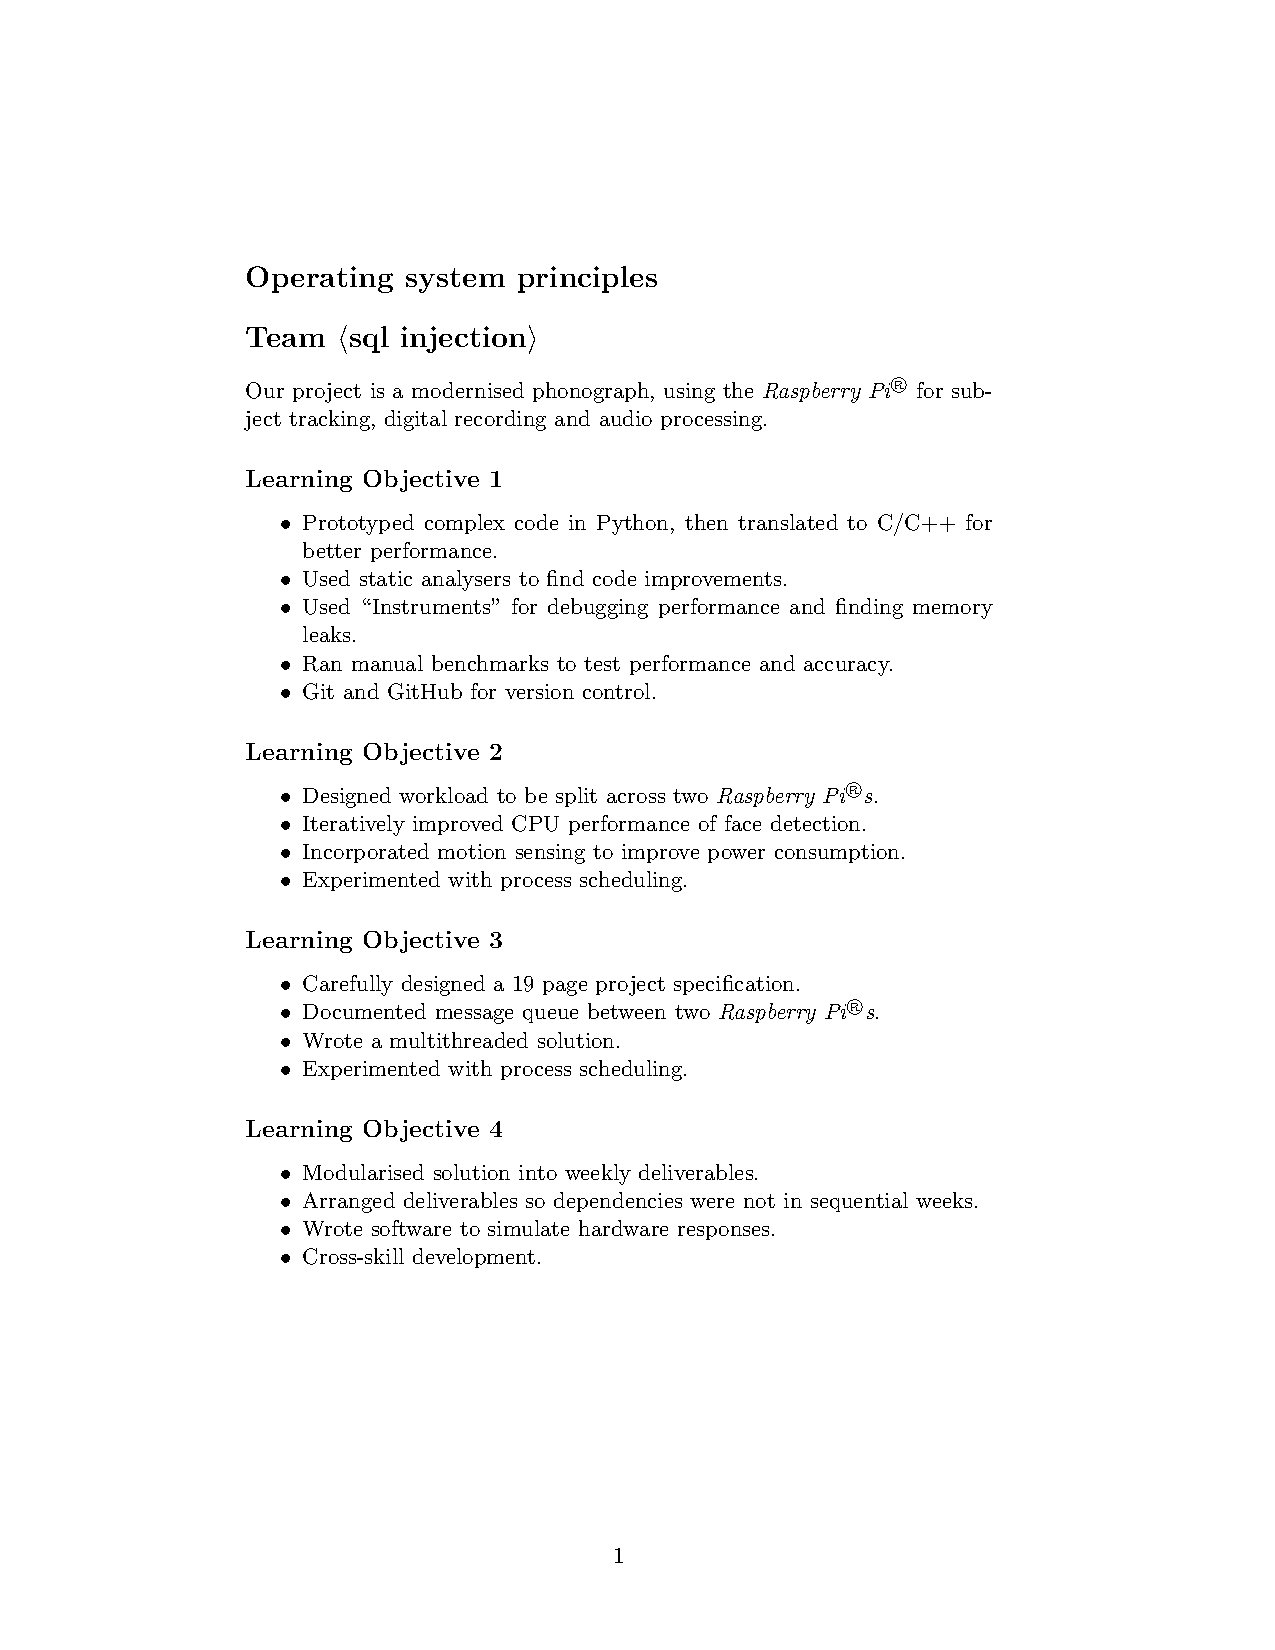
\includepdf[pages=-]{appendix/summary.pdf}



\chapter{Prototype Demonstration - Slides}
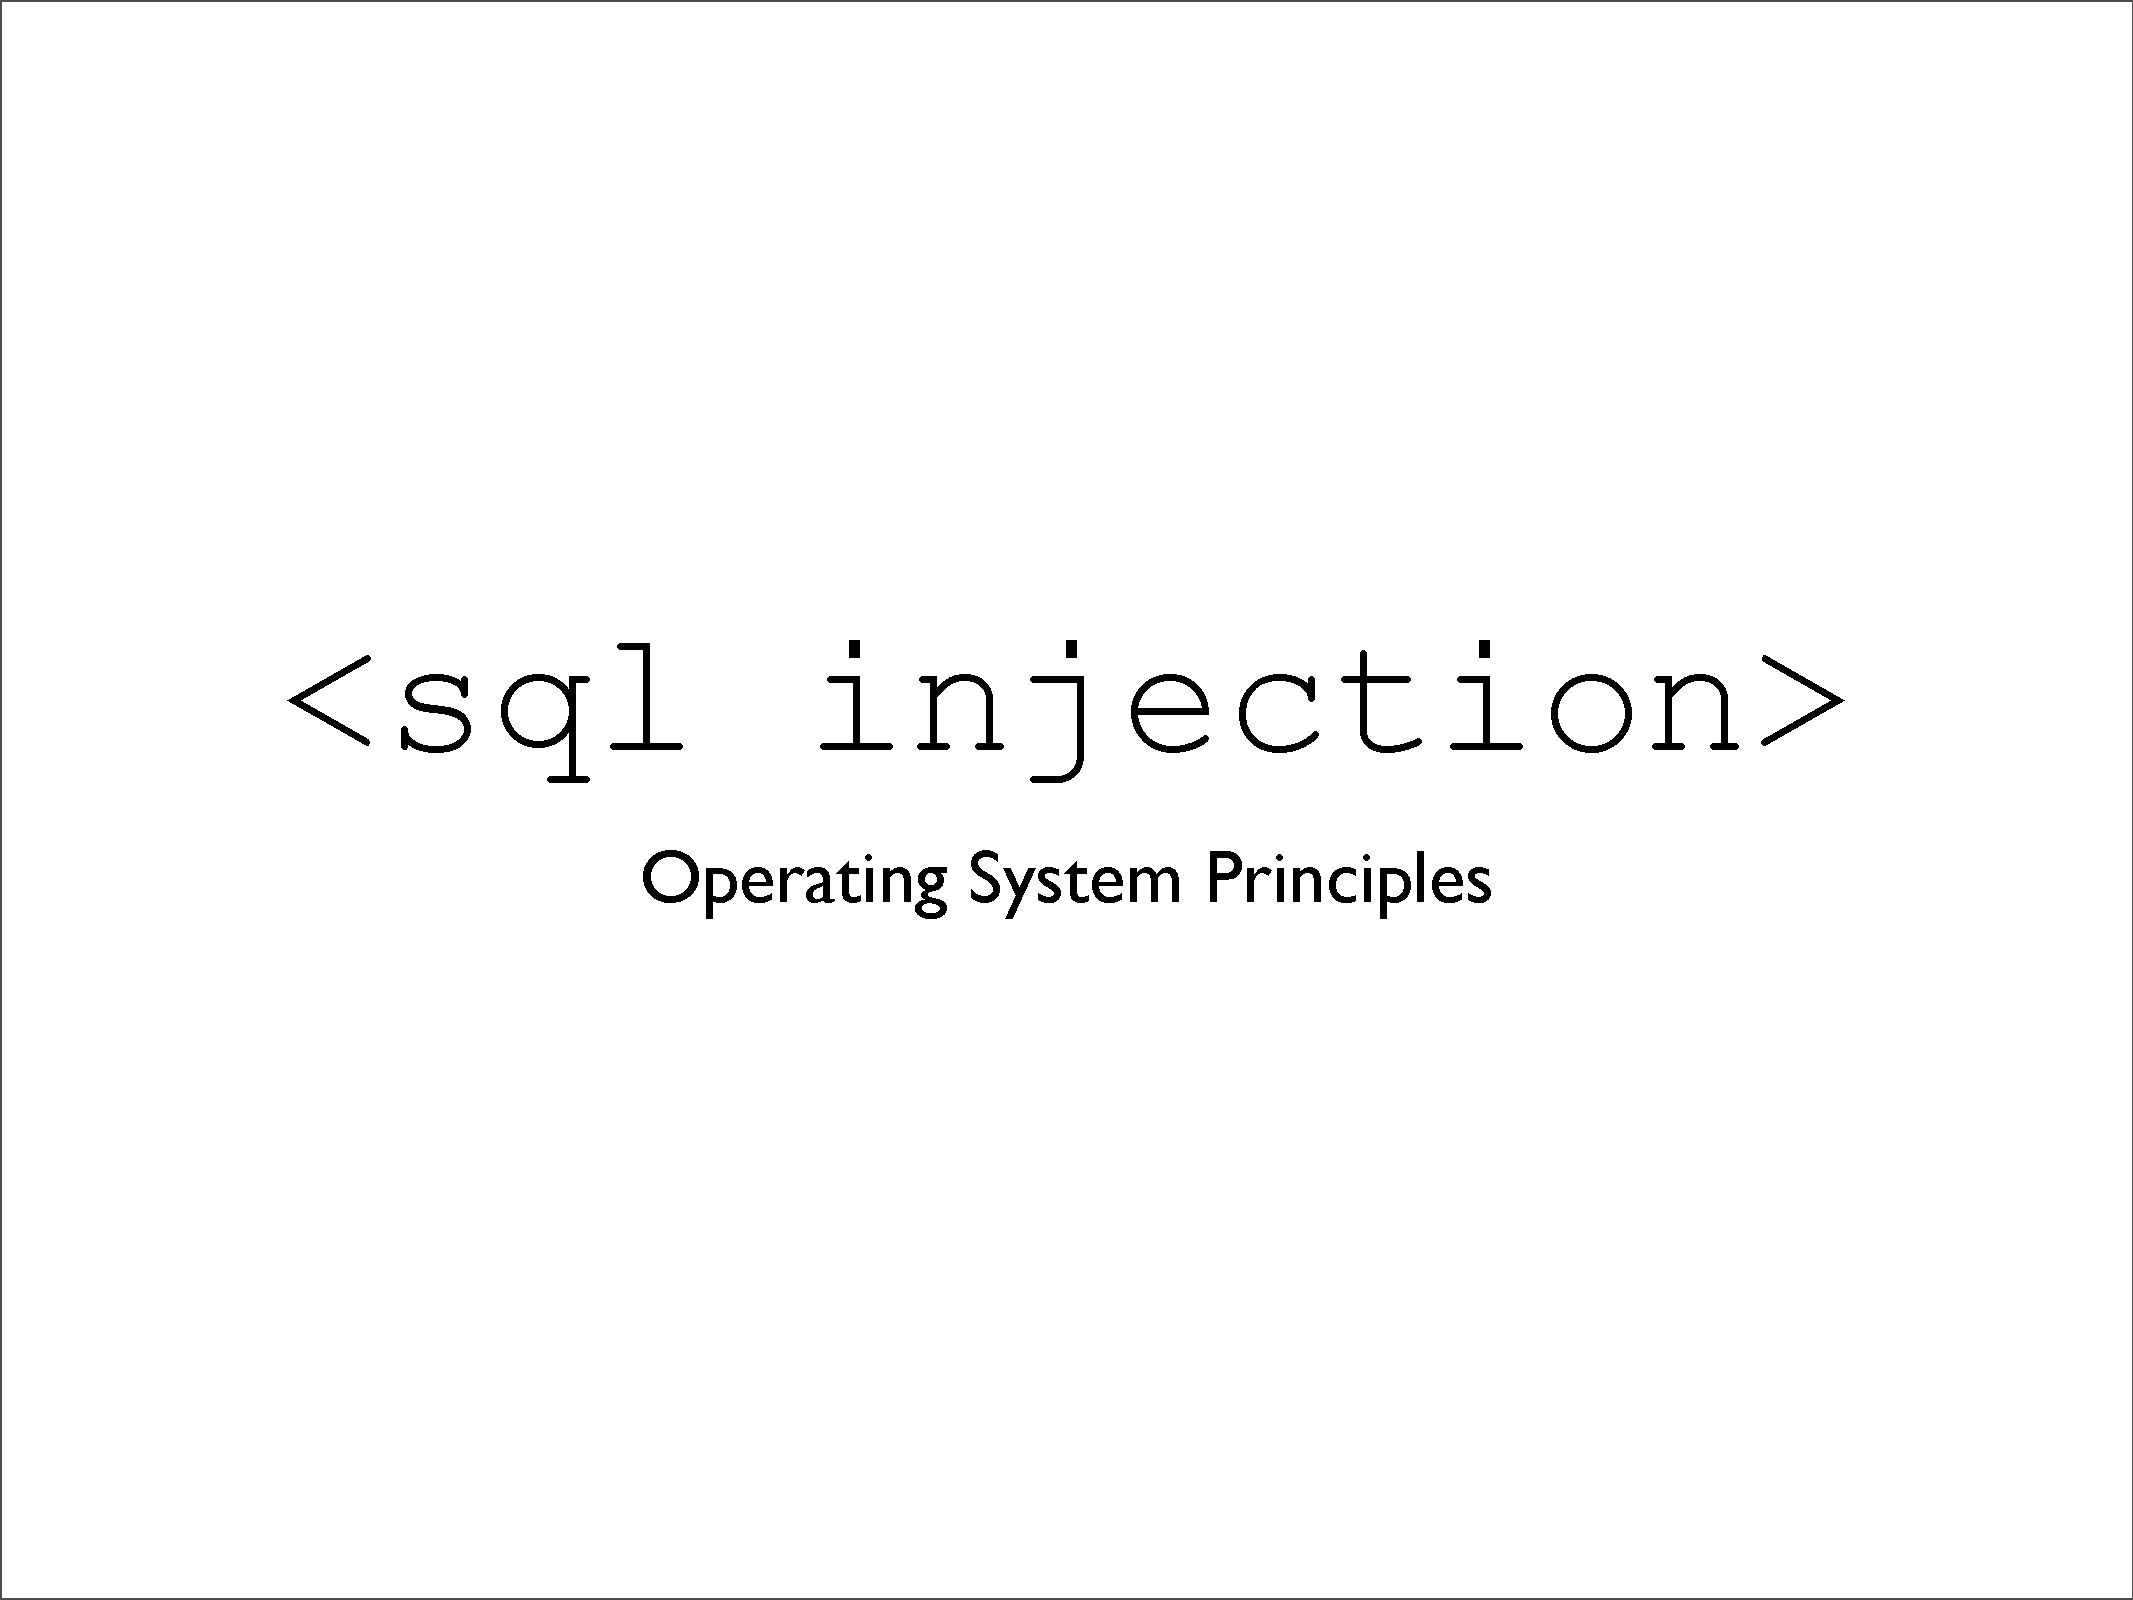
\includepdf[fitpaper=true,pages=-]{appendix/presentation.pdf}


\chapter{Project Specification}
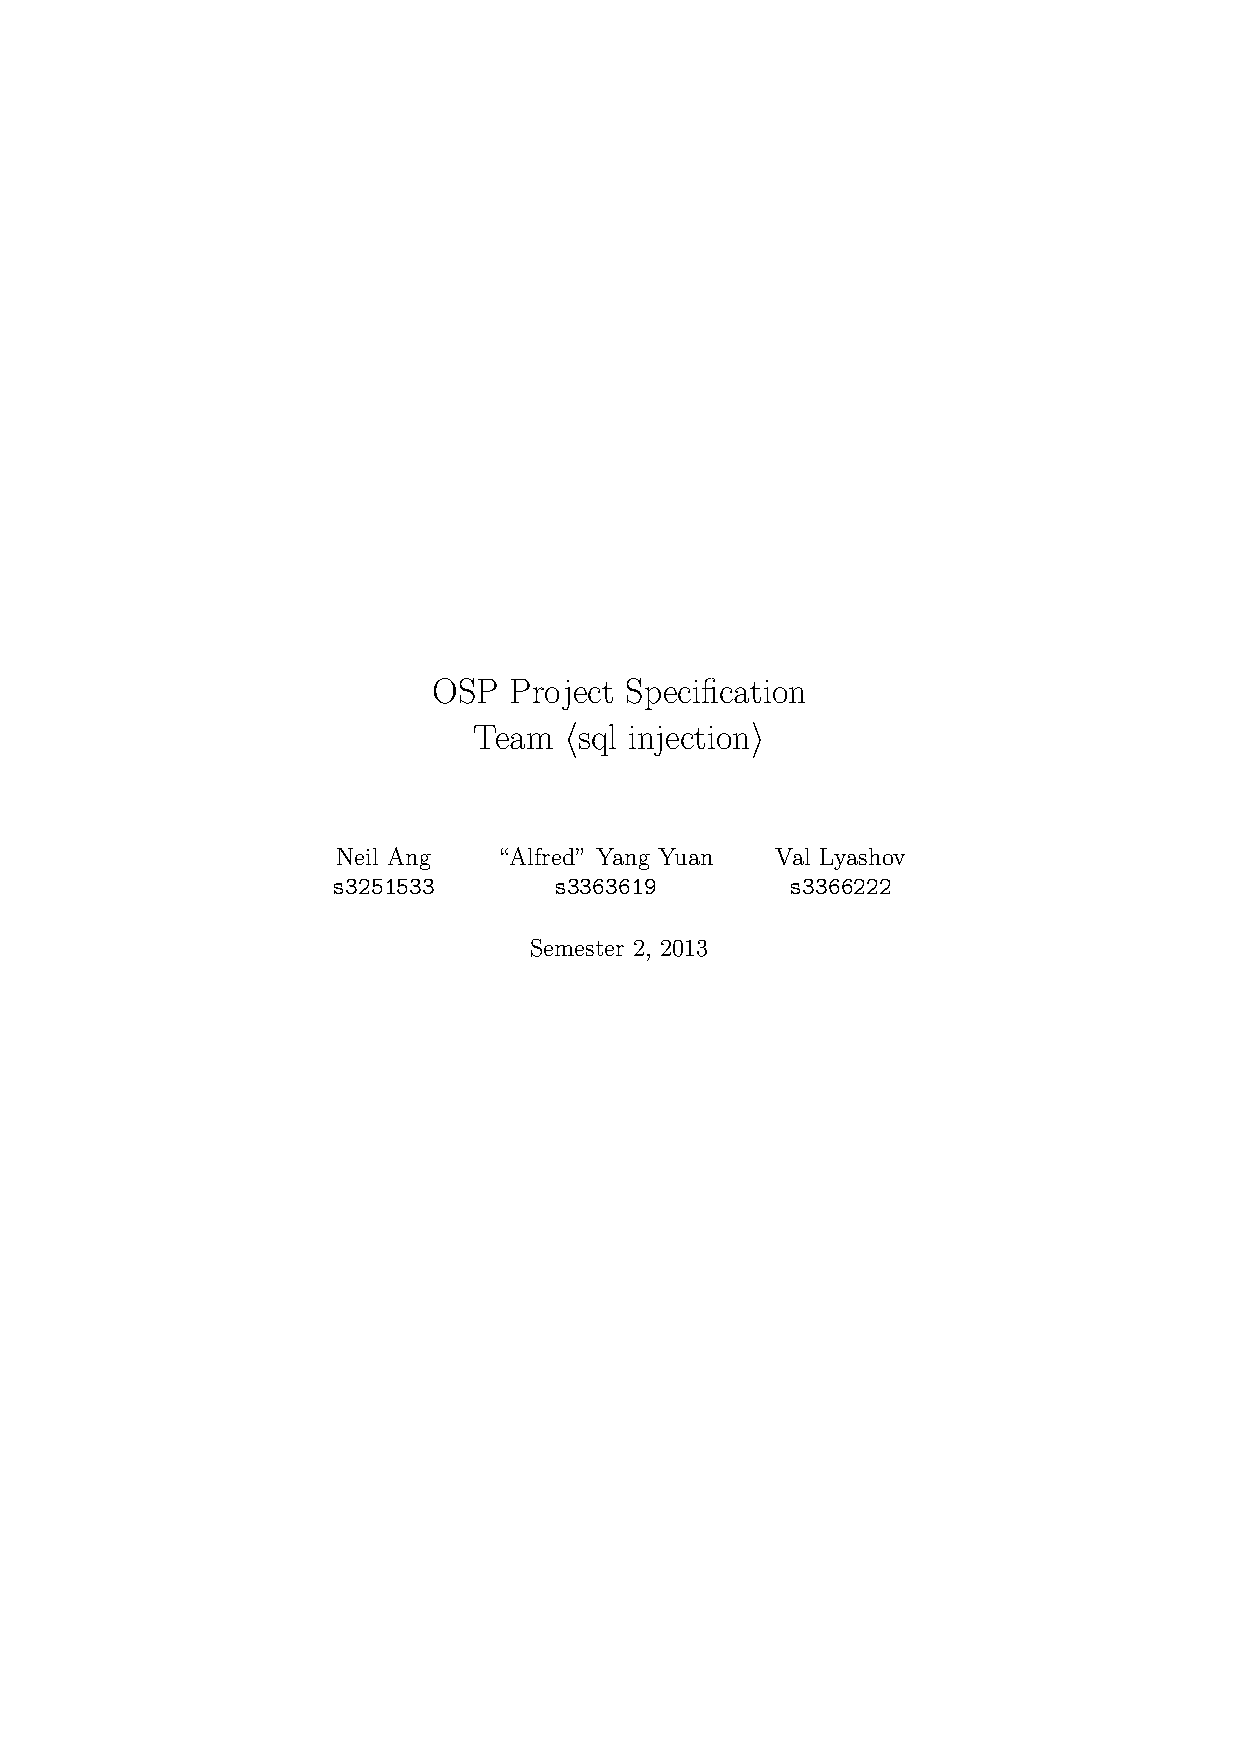
\includepdf[pages=-]{appendix/specification.pdf}



\end{appendices}

\nocite{*}
\printbibliography[heading=bibintoc]


\end{document}